\input{|"curl -L 'https://virginia.box.com/shared/static/9120uqo655t0kwesti7t3exa7zsgbwdq.tex'"}
%\include{article_header}
\title{Absence Makes the Ideal Points Sharper: Full-data IRT Models for Legislatures}
\usepackage{amsmath,amsthm, amssymb, latexsym}
\linespread{1.5}
\begin{document}
	
	\maketitle
	
	\begin{abstract}
		I put forward a Bayesian IRT model that can handle legislators absences as a separate category of data for determining legislator ideal points. The estimation uses the concept of a hurdle model to deflate the probabilities of legislator’s votes by the probability of absences. The model produces a single set of ideal points, but utilizes different parameters for bill absence points. Compared to existing approaches, this model tends to produce more moderate estimates of US Congresspeople’s ideal points because it can model roll-call votes where there are very few opposing votes. For parliamentary data, the model provides much more precise estimates, especially in legislatures with very high rates of absence. Additionally, the model can incorporate absentions as a middle category between yes and no votes for legislatures with high rates of abstentions.
	\end{abstract}
	
	Ideal point modeling of legislatures, and increasingly diverse kinds of social actors, has become an increasingly important part of empirical work in political science. However, most models of ideal points are based on binary outcomes that reflect yes and no votes (or positions) while all other actions are recorded as missing data. The argument for doing so is that the yes and no votes contain most of the information about legislator ideal points, and that incorporating other categories such as abstentions or absences would greatly complicate the estimation without adding much benefit. In relation to the first point, I present a model that uses Bayesian Markov Chain Monte Carlo (MCMC) estimation to handle the contingency inherent in the data. In relation to the second, I show in this paper that absences and abstentions do contain important information about legislator ideal points, a contention that has become more prominent in recent research.
	
	However, I depart from the discussion of ideal point models in this recent literature by treating absences and abstentions as additional data rather than as missing yes/no votes. This distinction, while somewhat technical, has important ramifications for modeling choices. If absences and abstentions represent missing yes/no votes, then the solution is to impute how a legislator would have voted if they had not either been absent or voted to abstain. Accomplishing this result is no easy feat because multiple imputation methods require that at some level the unobserved outcomes be random, or ignorable, relative to the observed outcomes (i.e., yes/no votes). Given that legislator behavior is usually strategic and not random, I argue that the requirements of multiple imputation are unlikely to be met without relying on additional parametric assumptions. 
	
	In this situation, the difficulty of multiple imputation is not a difficulty because the observed outcomes--absence and abstention--offer potential insight into ideal points. To this end, I have decided to incorporate absences and abstentions by adding them as outcomes within a standard item-response theory (IRT) ideal point model. While the ensuing model is more complicated than a traditional ideal point model, the model estimates a single set of ideal points, which means that the ideal points will be more precisely estimated than with a model that uses only yes or no votes. By treating absences and absentions as additional observations of legislator behavior, rather than as a statistical problem to be overcome, ideal point models can produce additional insight about legislators without requiring additional data collection.
	
	In this paper I first describe the current state of ideal point modeling with an attention to the growing awareness of the problem of absences and abstentions. I then present the model formally and offer simulation results to verify the model's performance. Then I examine two different empirical applications of the model, one drawn from data from the United States Congress and the second from the parliament in Tunisia's transitional democracy.
	
	\section*{Missing Data in Ideal Point Modeling}
	
	Following the pioneering work of \textcite{poole1997} and \textcite{jackman2004}, ideal point models have become a standard feature of the analysis of legislators and increasingly other political actors. The canonical ideal point model expresses legislator preferences as distances from a latent position in an $n$-dimensional policy space \parencite{enelow198} where the distances can be calculated either as Euclidean distances (IRT) or using the Normal distribution (i.e., the NOMINATE models), although both of these approaches tend to offer very similar estimates  \parencite{carroll2009}. A fully Bayesian analysis such as \textcite{jackman2004} is able to analyze virtually all bills, but whether done in a frequentist or Bayesian framework, the focus has remained on ideal points as representations of yes/no votes.
	
	Recently there has been criticism of these approaches because the ideal points that are estimated may not be an accurate measure of a legislator's ``true" ideological stance \parencite{krehbiel2014,Caughey2016,brauninger2016}. Statistically speaking, the ideal points are the dimension of variance that best explains the observed outcomes, so there is no easy way to know whether the ideal points refer to a legislator's ideological inclinations or more to his or her political strategies. For the model I present, however, this latter interpretation is more helpful because it makes it clear why data on absences and abstentions would be important to include. To the extent that voting can be represented in a unidimensional space, this space should be able to account for the full range of legislative behavior. The ideal point may properly refer to a legislator's firm political convictions or it may reflect their desire to appear more moderate/liberal/conservative for tactical reasons. Regardless, these ideal points are by definition the lowest-error explanation of observed behavior, and for that reason they are worth studying, even if as latent variables we cannot identify with complete certainty what social concepts they correspond to.
	
	Building on this work, political scientists have begun to look at alternative sources of data about ideal points beyond the collection of yes and no votes. A growing literature uses data generated outside of the legislature, whether via Twitter \parencite{barbera2015}, through political donations \parencite{bonica2014}, or through the legislator's prior history as a state representative \parencite{shor2011}. Most recently, \textcite{brauninger2016} and \textcite{rosas2015} have proposed methods for including abstentions and absences in parliamentary rollcall voting, while \textcite{powell2016} has presented new data on Congressional absences that shows how different types of absences may provide varying signals of legislator partisanship.
	
	What remains a lacuna, however, is how to incorporate bsences and abstentions in the standard rollcall vote model that still serves as a benchmark for much of applied work in legislatures. Both of the extant IRT and NOMINATE approaches drop absences and absentions from their data, which means that the ideal points ignore any information contained in this part of the dataset. Properly speaking, the standard models are only defined over the subset of rollcall voting that comprises yes and no votes. It is not that these models are in any sense incorrect or useless, but rather that their domain is limited to the binary relationship of opposing votes on bills. However, it would seem that given the interest in obtaining new methods of ascertaining ideal points, this discarding of data is not an ideal method.
	
	
The methodology that has been used so far to address this problem is multiple imputation because absences and abstentions are coded as missing values. Multiple imputation involves estimating the distribution of possible yes or no votes to replace all of the absences and abstentions in the data. Crucially, for this method to work, the probability of an unobserved response must not depend on the value of that unobserved response \parencite{rubin2002}. 	In the broader IRT field there are extant approaches to handling missing data that follow from \textcite{rubin2002}'s framework. \textcite{mislevy2016} provides a helpful summary of these approaches by showing how ignorability of missing data, and the crucial missing-at-random (MAR) assumption, depends on the relationship between the person ``ability" parameters (i.e., legislative ideology) and the item parameters (i.e., bill yes/no points). However, he concludes that if the missing data is due to ``intentional ommission" or to ``examinee choice", then no extant IRT missing-data model is able to meet the MAR assumption (p. 192). However, virtually all recorded legislative actions are intentional at some level. To correctly impute votes, we would need to imagine a counter-factual world in which some divine force forced a legislator to show up and then to vote either yes or no. While this counterfactual is plausible in some situations, such as if a legislator suffered some kind of accident preventing them from showing up, in general it is not plausible to impute this counterfactual.
	
	However, this approach can be used within the context of a specific model specifying how the counterfactual could occur. \textcite{rosas2015} is the first to apply this theoretical approach to rollcall voting data via an imputation model of legislative behavior framed in terms of disagreement between a party member and the party's official position.  As \textcite{rosas2015} point out, in the case of rollcall vote data, the assumption that absences and abstentions can be thought of as a plausibly random distribution yes/no votes is unlikely to be true. In \citeauthor{rosas2015}'s model, yes and no votes are imputed based on whether a party member is in agreement with his or her party given the assumption that, conditional on knowing whether a party member is in disagreement, the ensuing decision to vote yes or no only depends on observed ideal points \parencite{rubin2002}, and hence is imputable. This model provides a compelling account of how a legislator may decide to abstain in a vote; however, the model's applicability is also limited to this specific counterfactual. For example, \citeauthor{rosas2015} collapse both absences and abstentions into a single category because in their framework these actions are equal signals of party disagreement, but this may not be applicable to other situations of legislative behavior.
	
	By comparison, the model that I propose should apply to abstention and absence data more broadly, although it does not provide special insight into intra-party dynamics as \textcite{rosas2015} do. The main difference is that I do not attempt to impute observations. Rather, the model I present in this paper treats absences and abstentions as additional data that can estimated jointly with the standard models to improve the accuracy of ideal points. By treating absences and abstentions as strategic actions, I can directly incorporate them into the model as additional evidence of legislators' ideal points. This change in focus allows for a complete-data IRT model that uses every possible category of votes (absent,abstain,yes,no) in legislative roll-call datasets.
	
	
	
	\section*{Absence-Inflated Hurdle Model}
	
	To handle the full range of strategic outcomes in legislative data, I propose embedding two IRT equations inside of a hurdle model. A hurdle model, which is similar to a zero-inflated model, accounts for one-way censoring in data by separately modeling a probability that an observation belongs to either the hurdle or to the full IRT model. 
	
	I begin with an IRT ordered logit model, which is known as a rating-scale model in the IRT literature.\footnote{A rating-scale model has fixed cutpoints for the entire data and matches the parameterization of the commonly-used ordered logit model. The graded-response model, on the other hand, estimates separate cutpoints for each bill. While it is an interesting extension of the basic model, it is not considered in this paper, although it can be estimated in the \texttt{idealstan} R package.} The $K$ category vote outcome $_k$ can be modeled as a likelihood function $L(\cdot)$ of $I$ legislator ideal points $x_i$, $J$ bill discrimination parameters $\beta_j$ and $J$ bill intercepts $\alpha_j$. Each equation is put inside $\zeta(\cdot)$, which represents the logit function. Formally, the full likelihood is:
	
					\[
	L(\beta,\alpha,x|Y_{k}) = \prod_{n}^{i=1} \prod_{m}^{j=1}
	\begin{cases} 
	1 -  \zeta(x_{i}'\beta_j - \alpha_j - c_1) & \text{if } K = 0 \\
	\zeta(x_{i}'\beta_j - \alpha_j - c_{k-1}) - \zeta(x_{i}'\beta_j - \alpha_j - c_{k})       & \text{if } 0 < k < K, \text{ and} \\
	\zeta(x_{i}'\beta_j - \alpha_j - c_{k-1}) - 0 & \text{if } k=K
	\end{cases}
	\]
	
	The use of $K$ ordered outcomes allows the model to incorporate abstentions as a third category between yes and no votes. Because the cutpoints are estimated from the data, the actual width of the utility apportioned to voting in each category will vary from dataset to dataset. In the Bayesian framework with priors on variables described later, there is no risk of cutpoint collapse because any bills with zero abstentions will simply default to the prior.
	
	The bill intercepts also have a slightly different interpretation in this model. The intercept for each bill is actually $\alpha_j + c_k$ for all $K$ so that in effect the bill has an intercept for each category of vote outcome. Otherwise, however, the estimated parameters are interpreted identically to the standard IRT model \parencite{jackman2004}. The $x_i$ represent legislator ideal points and the bill midpoints (i.e., the line of indifference for each vote outcome) are equal to $\frac{\alpha_j + c_{k-1}}{\beta_j}$. Thus for a rollcall voting model with three distinct outcomes, yes, no and abstain, there will be two lines of indifference (or equiprobability contours) for each bill that separate legislators into groups that are more or less likely to vote in each vote category. For the binary case in which $K=2$, the cutpoints collapse into the bill intercepts and a standard binary logit model is estimated.
	
	In order to model absences, this standard IRT model is embedded within a hurdle framework, which is similar to the zero-inflated models popular with handling over-dispersion in count data. We assume that the probability that a legislator is absent is equal to $r$ and the probability that the legislator shows up to vote is equal to $1-r$. The probability $r$ is itself modeled as a binary IRT model in which the ideal points $x_i$ are shared with the vote equation while the bills receive separate parameters $\gamma_j$ for discrimination and $\omega_j$ as intercepts. Functionally, this means that the probability of any vote $K$ is decreased proportionally as the probability of absence $r$ increases. A legislator will only vote if the hurdle of strategic absence is overcome. That is to say, not only does each bill have a point in a voting ideal space, it also has a point in an absence ideal space that is also relative to the legislators' own ideal points.
	
	The combined model is as follows:
	
		 \[
	L(\beta,\alpha,X,Q,\gamma,\omega|Y_{k},Y_{r}) = 
	\prod_{n}^{i=1} \prod_{m}^{j=1}
	\begin{cases}
	\zeta(x_{i}'\gamma_j - \omega_j ) & \text{if } r=0, \text{ and} \\
	(1-\zeta({x_{i}'\gamma_j - \omega_j}))L(\beta,\alpha,X|Y_{k1}) & \text{if } r=1
	\end{cases}
	\]
	
	Substantively, the additional bill parameters $\gamma_j$ and $\omega_j$ represent the position in the ideal point space of the salience of a particular bill. $\omega_j$ refers to the average probability that legislators will be absent on a given bill, while $\gamma_j$ reflects the position in which the bill is pointing in the ideal space, i.e., whether a bill is liberal or conservative. Unlike in standard IRT models,the $\gamma_j$ and $\beta_j$ discrimination parameters are unconstrained to allow a bill to have either a conservative or liberal polarity in the ideal point space. 
	
	The addition of parameters, and the dependent relationship between the hurdle model and the vote model, makes estimation more challenging. Estimating the parameters with Bayesian MCMC requires the usual identification restrictions on parameters \parencite{jackman2004,gelman2005}, but the additional parameters may require further constraints in order to identify the model. There is no easy or straightforward method to identify this model as it depends in part on the presence of information in the model about both bills and legislators. However, the usage of usual identification methods, such as constraining polarity and fixing parameters is able to identify most models.\footnote{In the R package \texttt{idealstan} I provide methods for automatically identifying models through the use of variational Bayesian inference}
	
	The following priors are put on all of the parameters:
	
	\begin{align*}
		c_k - c_{k-1} &\sim N(0,5)\\
		\gamma_j &\sim N(0,5)\\
		\omega_j &\sim N(0,5)\\
		\beta_j &\sim N(0,5)\\
		\alpha_j &\sim N(0,5)\\
		x_i &\sim N(0,1)
	\end{align*}

	
	Essentially, all parameters are given a weakly informative $N(0,5)$ prior (five is a large number on the logit scale). For scale identification purposes, the $x_i$ ideal points are given a $N(0,1)$ prior. In addition, one each of the $\alpha_j$ and $\omega_j$ intercepts are fixed at zero in order to prevent scale shifts in the parameters. A prior is put on the difference between the cutpoints $c_k$ rather than on the cutpoints themselves because it is difficult to affix concrete values to cutpoints a-priori, although the differences between cutpoints can be weakly identified. The prior on the cutpoints prevents cutpoint collapse so that it is not necessary to have a certain number of abstentions for each bill, while the bias of using a weakly informative prior is minimal.
	
	To show how the model performs, I simulated data of 100 legislators and 100 bills. For the purposes of identification, I constrained the signs of ten legislators to identify the scale, and used vague priors on the other parameters as mentioned above. Estimation of the model was through an R package \texttt{idealstan} that provides this model along with other absence-inflated IRT ideal point models for both ordinal and binary data. The results of the simulation are shown in Figure \ref{sim_results}.
	
	\begin{figure}
		\caption{True and Estimated Values}\label{sim_results}
	\end{figure} 
	
	
	
	\section*{Empirical Applications}
	
	As an empirical application of the model, I look at two rollcall datasets, one from the 114th Senate and the second from a transitional democracy, Tunisia. For both datasets I use existing R packages, \texttt{wnominate} and \texttt{pscl}, to obtain ideal scores using the W-NOMINATE and IRT methods respectively. I then estimated absence-inflated models for both datasets, a binary IRT for the Senate data and an ordinal IRT for the Tunisian data. I did not use an ordinal model for the Senate data because there were only a handful of abstentions in the 114th Senate, and estimating cutpoints for abstention would make little difference to the model. 
	
	\subsection*{US Congress}
	
	The estimation results for the 114th Senate show that overall the absence-inflated model and both \texttt{ideal} and W-NOMINATE correlate very highly, as might be expected given the relatively low rates of absence. Figure \ref{compare_con} reveals that the models tend to diverge only in the tails of the Republican and Democrat parties. Furthermore, although the absence-inflated model is structurally more similar to \texttt{ideal} in that it is based on an IRT framework, for some legislators the absence-inflation model is closer to W-NOMINATE's estimate. 
	
	\begin{figure}
		\centering
		\caption{Comparison of Ideal, W-NOMINATE and Absence-Inflation Models for 114th Senate}\label{compare_con}
			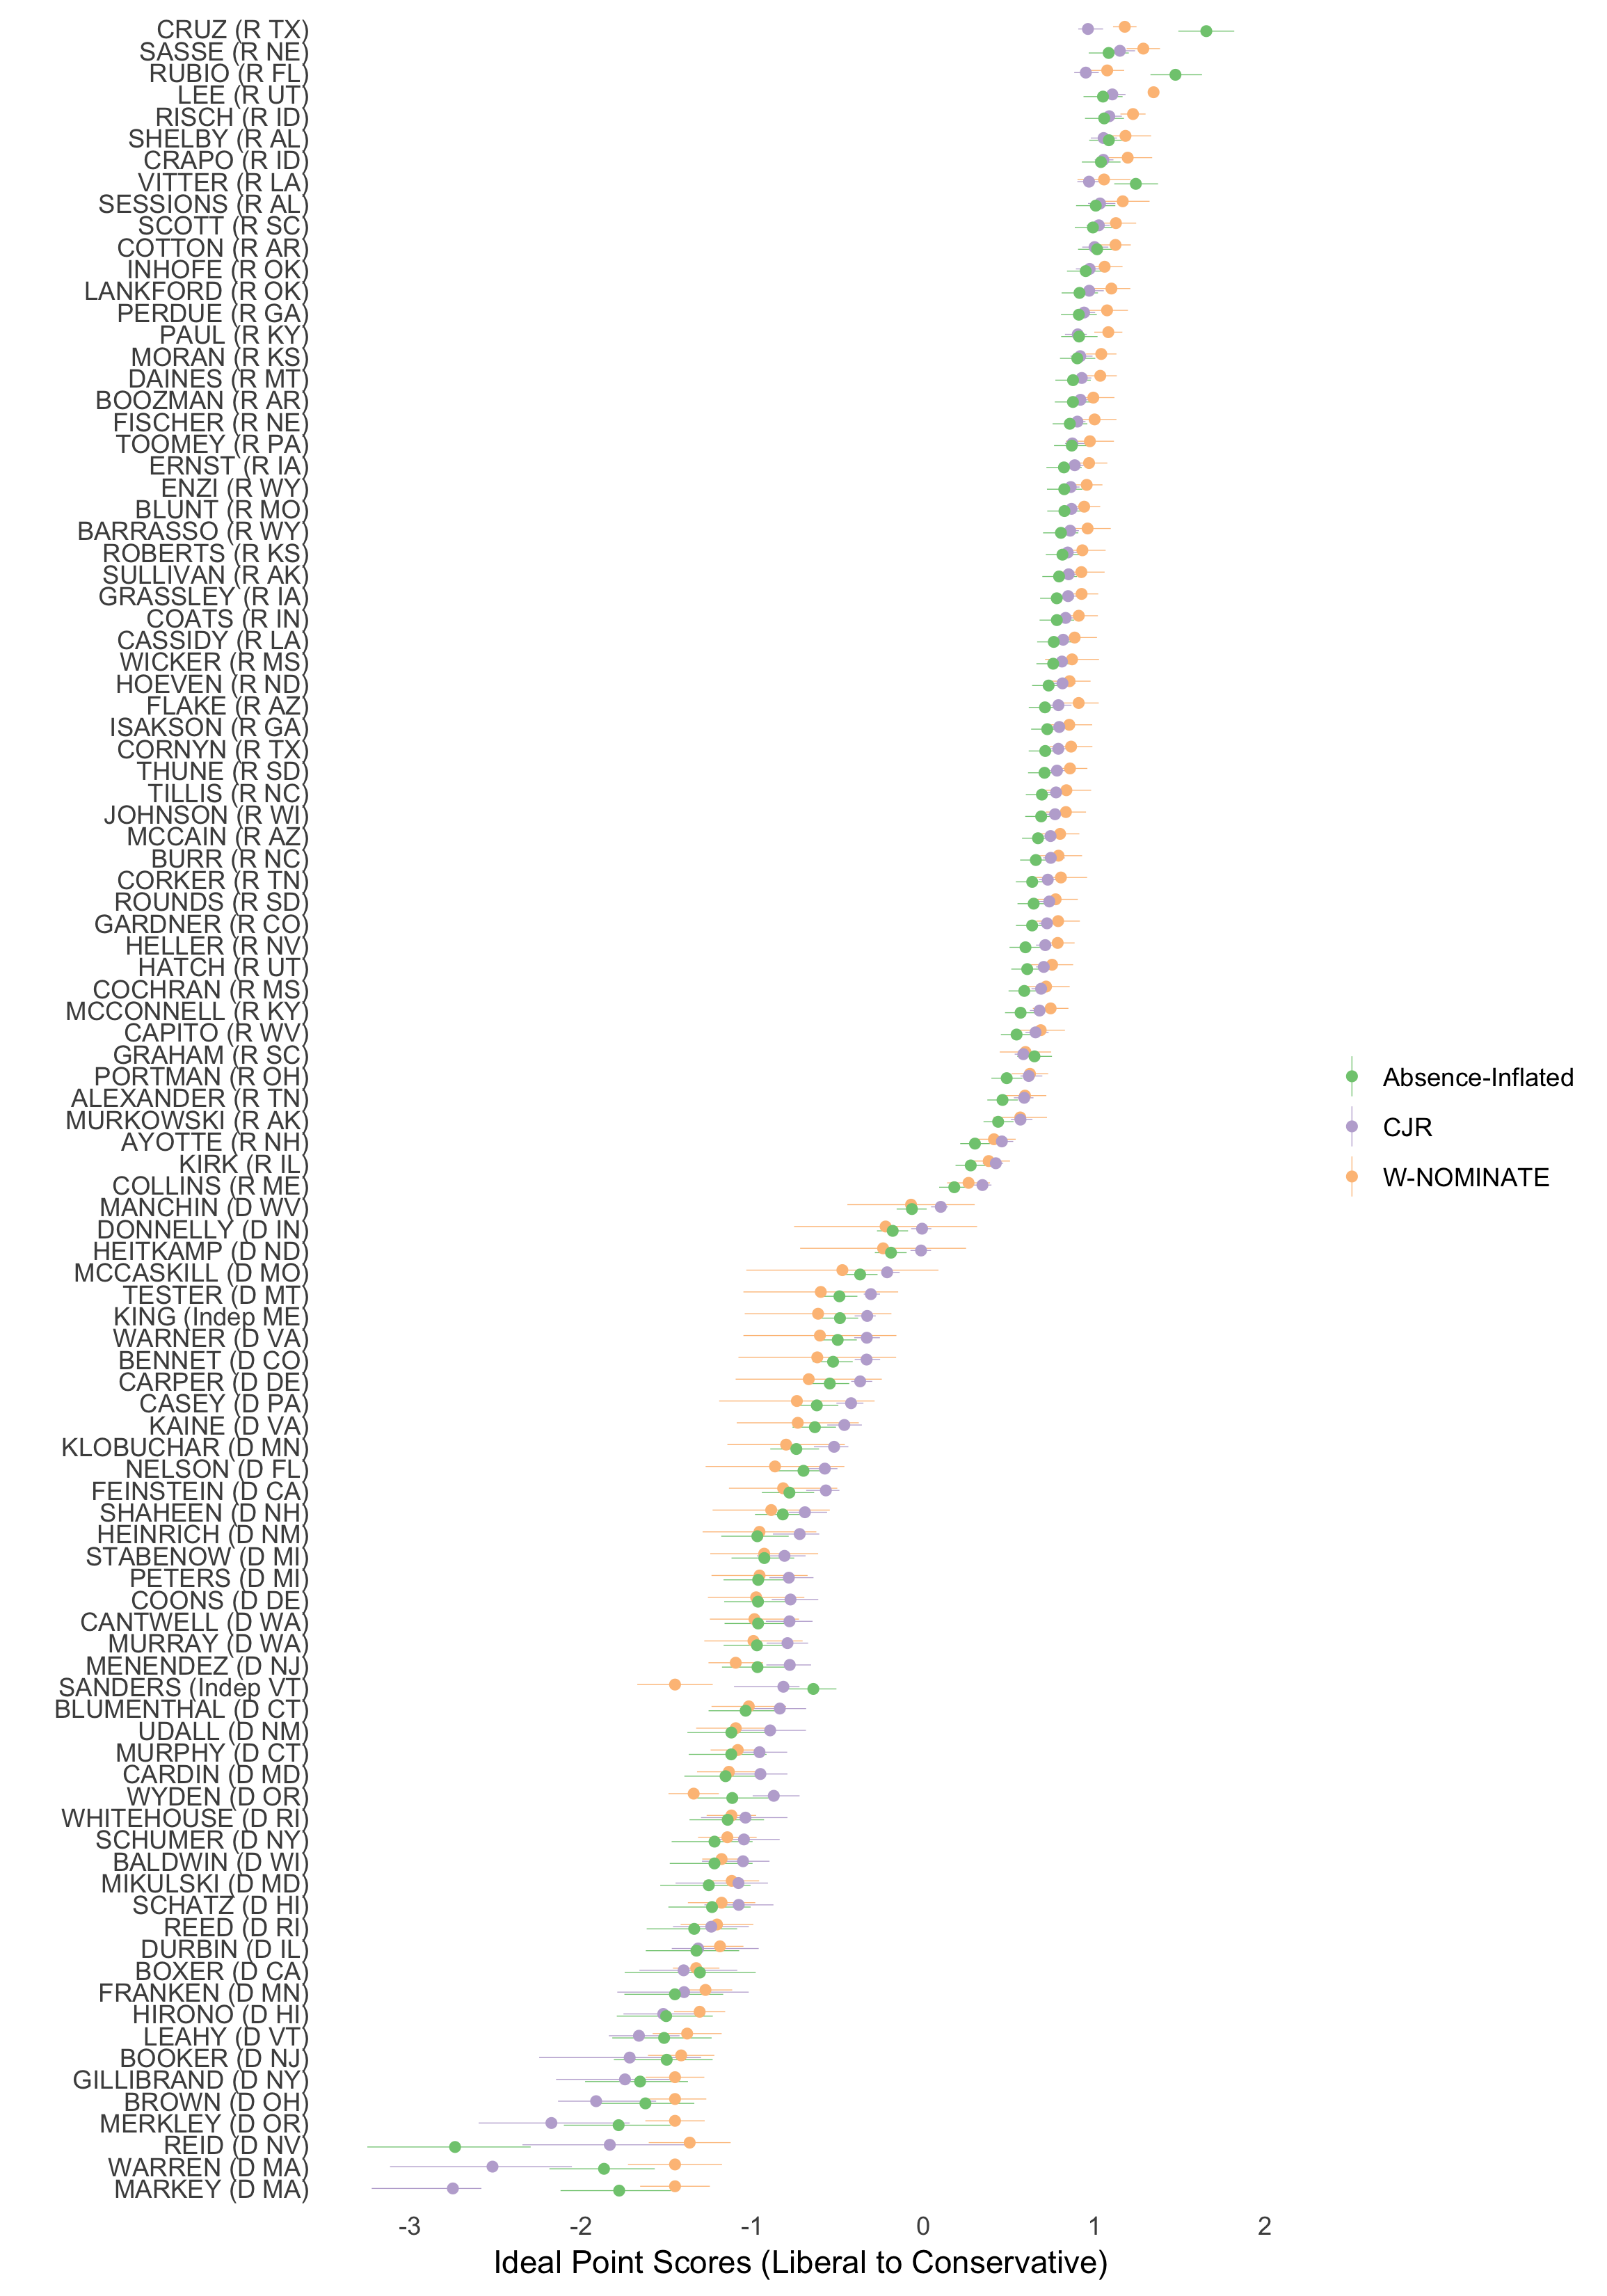
\includegraphics[width=\linewidth]{all_perf}
	\end{figure}
	
	Figure \ref{compare_con} shows that the standard models of \texttt{ideal} and W-NOMINATE are quite accurate at capturing ideal points despite the fact that these models drop absences. The close correlation between the scores shows that even if the assumptions of these models are not met, the resulting estimates are still very usable because the low number of absences ensures the model is still a close approximation of reality. However, as may be expected, the estimates diverge for those legislators who have higher rates of absence. For the 114th Senate, these are primarily Senators who were competing in the presidential primaries: Bernie Sanders, Ted Cruz and Marco Rubio. In fact, the absence-inflation model shows Ted Cruz and Marco Rubio as the most conservative senators in the data set, which is likely because Cruz and Rubio made sure they showed up for votes that mattered to the conservative Republican base during the primary season.
	
	\begin{figure}
		\centering
		\caption{Rank Changes for 114th Senate}\label{rank_sen}
		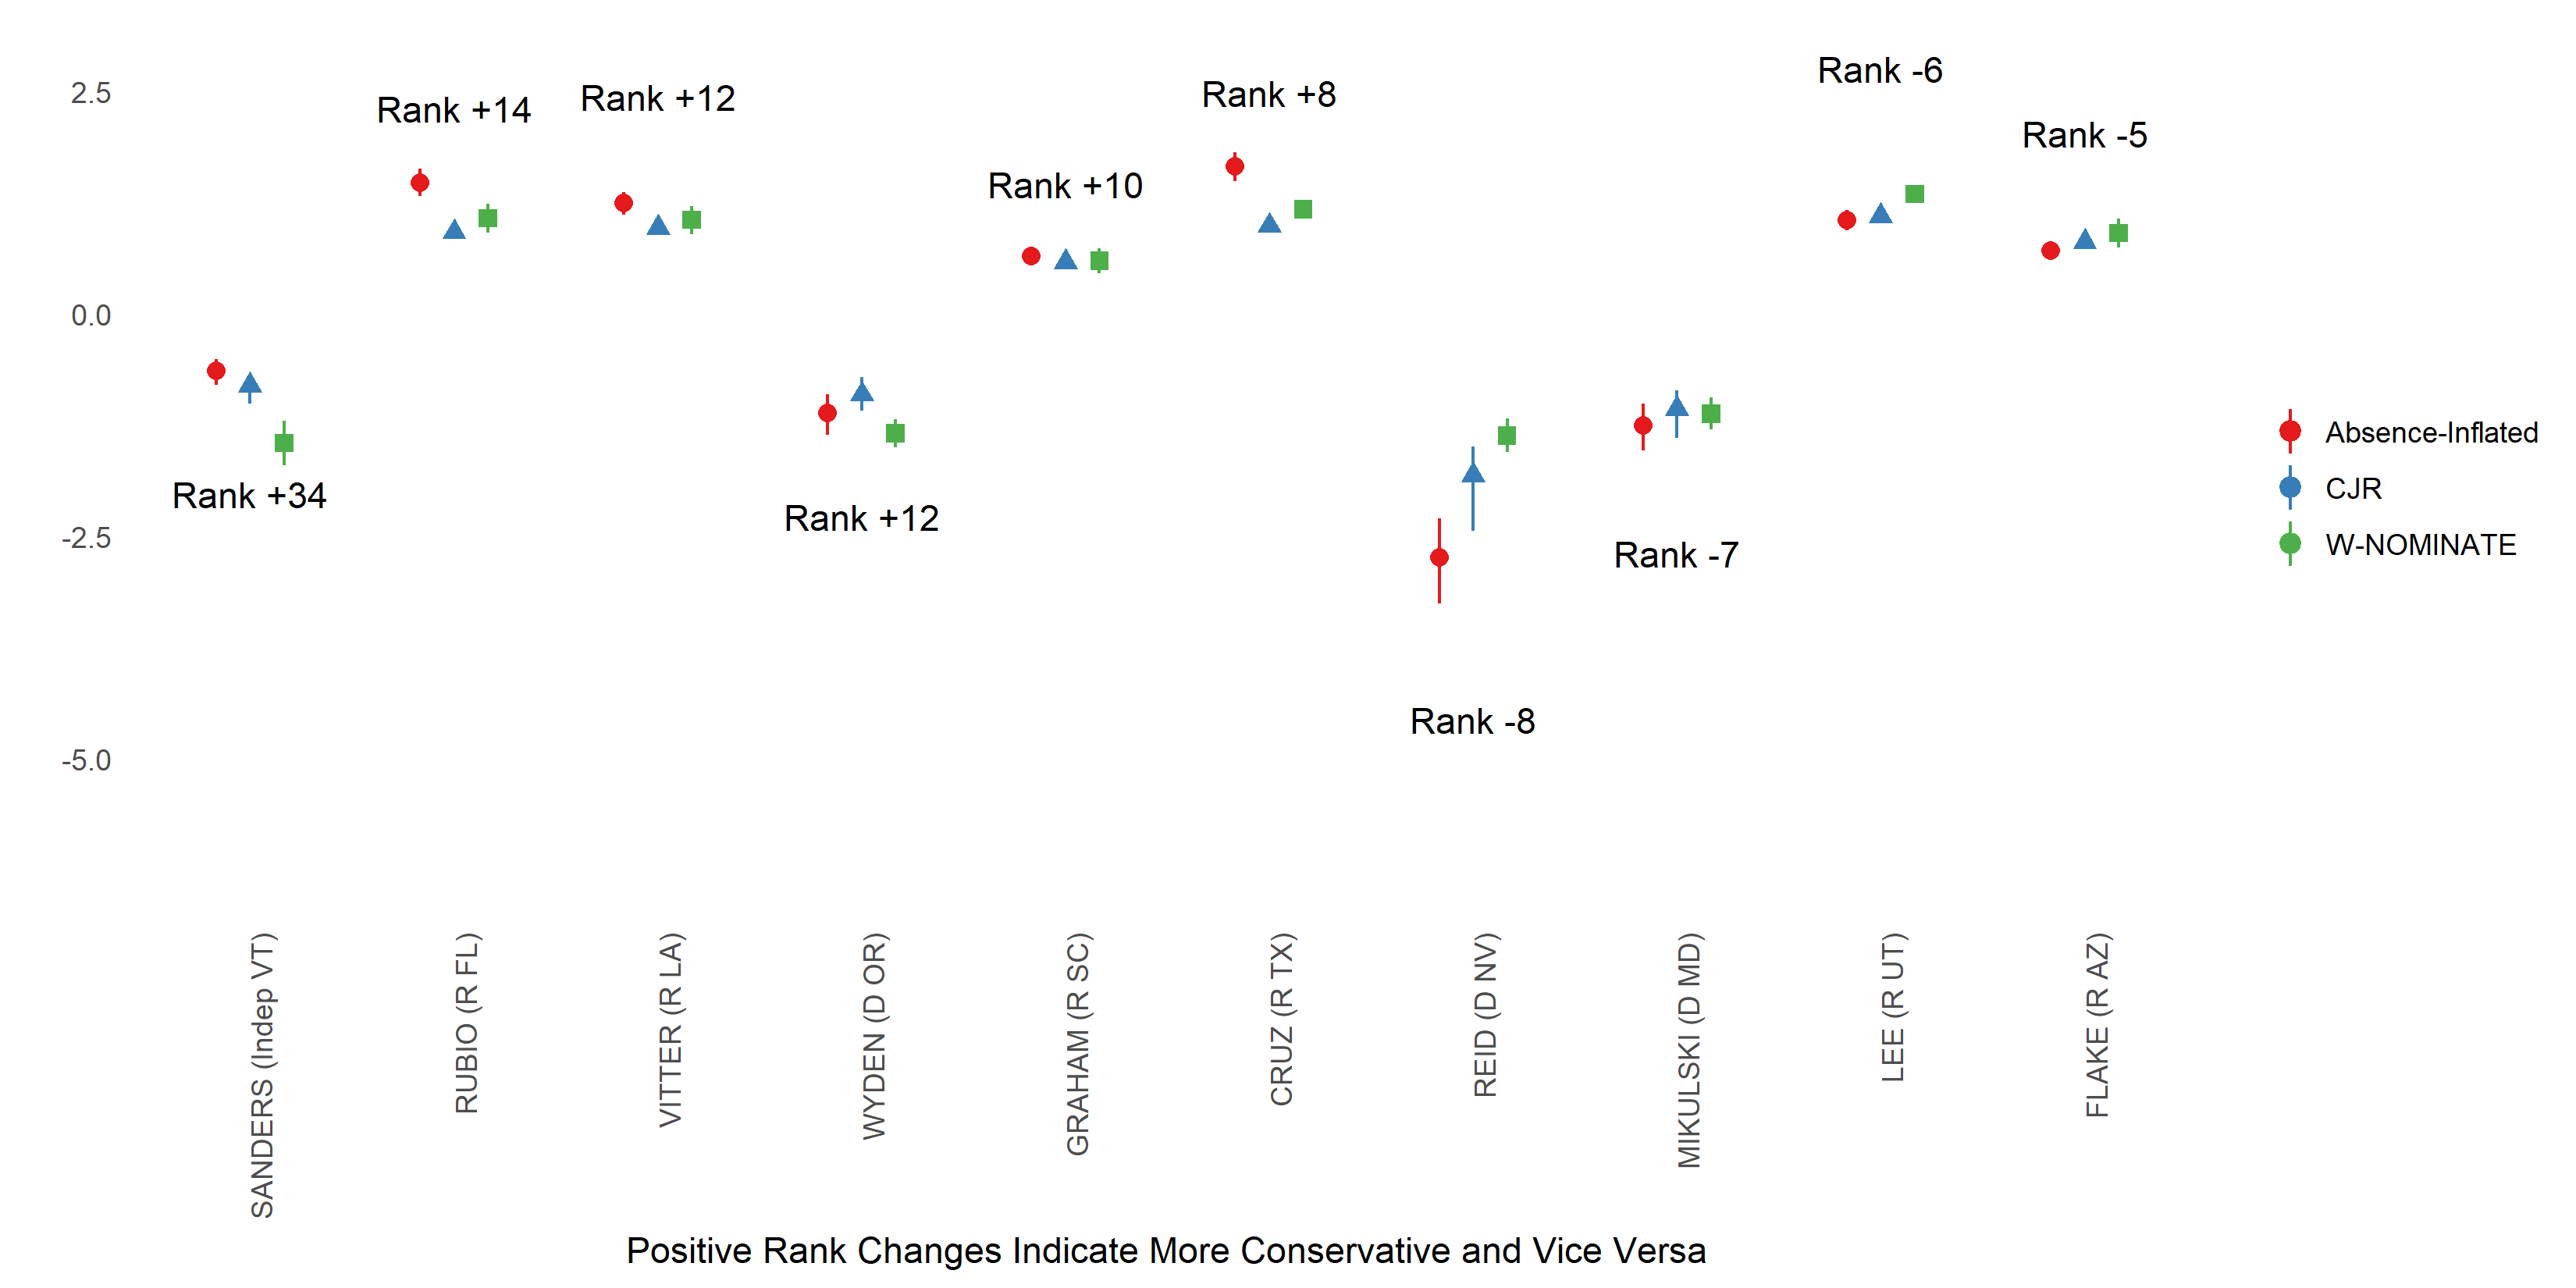
\includegraphics[width=0.8\linewidth]{big_diff}
	\end{figure}
	
	To track these changes within models, I show in Figure \ref{rank_sen} the largest changes in ranks between the absence-inflated model and the two standard models. Positive rank changes in the figure indicate a senator became more conservative as a result of having his or her absences included in the ideal point estimation. In some cases, such as with Bernie Sanders, the absence-inflated model is closer to the IRT-based \texttt{ideal} than the normal utility W-NOMINATE. But with Ted Cruz, Marco Rubio, and Harry Reid, who retired at the end of 114th Congress, the absence-inflated model is markedly different. With all three senators, the absence-inflated model shows the moving towards the ideological extremes. This is likely because all three Congresspeople had an incentive to only show up to bills for which their absence points were relatively polarized: for Cruz and Rubio, pleasing the conservative base, and for Reid, a chance to live out his ideological principles with conviction before retirement.
	
	\subsection*{Tunisian Parliament}
	
	\section*{Discussion}
	
	\section*{Conclusion}
	
	\section*{Appendix}
	
	\section*{References}
	
	
	
\end{document}